\documentclass[a4paper,12pt]{article}

\usepackage{tikz}
\usepackage[utf8]{inputenc}
\usepackage{amsmath}
\usepackage[australian]{babel}
\usepackage{fontenc}
\usepackage{graphicx}
\usepackage[euler-digits]{eulervm}

\title{Complicated Boundary-Value Problem}
\date{15 September, 2023}
\author{William McLean}

\begin{document}
\maketitle
\begin{center}
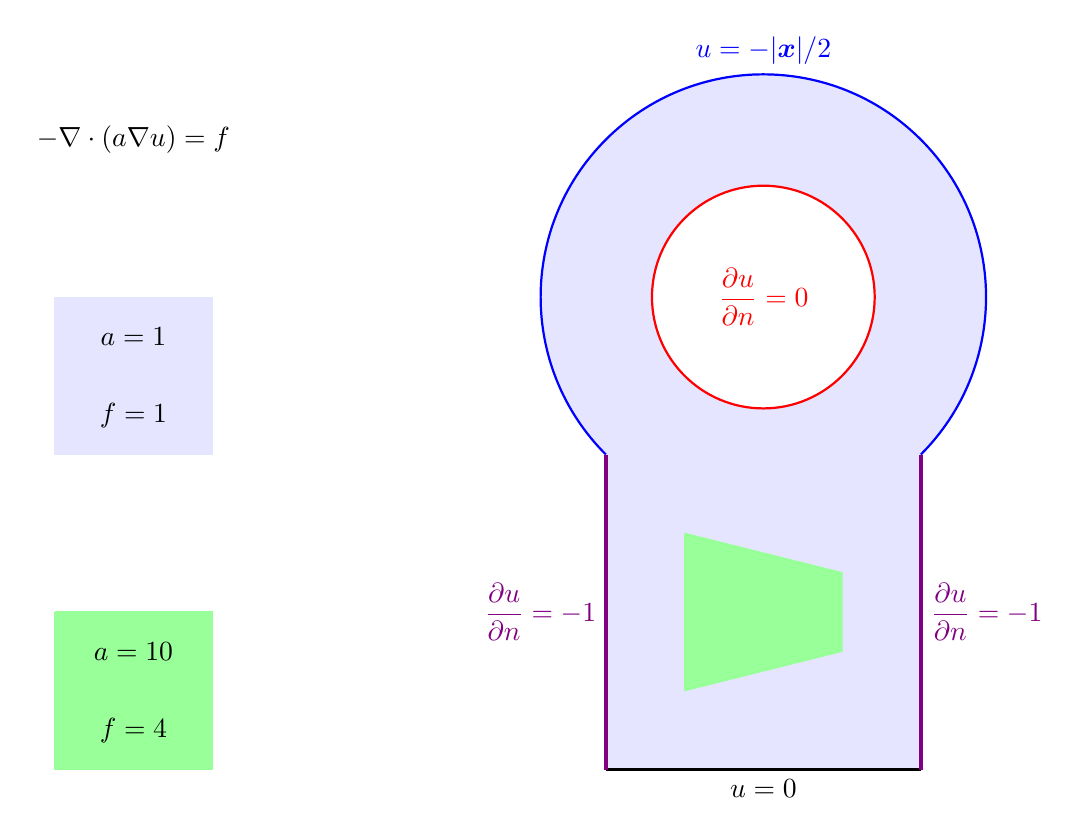
\begin{tikzpicture}[scale=2.0]
\path[fill=blue!10] (-1,0) -- (-1,-2) -- (1,-2) -- (1,0)
arc [radius=sqrt(2), start angle=-45, end angle=225];
\draw[blue,thick] (1,0)
arc [radius=sqrt(2), start angle=-45, end angle=225];
\draw[red,thick,fill=white] (0,1) circle [radius=sqrt(2)/2];
\draw[green!40,fill=green!40] (-0.5,-0.5) -- (-0.5,-1.5) --
(0.5,-1.25) -- (0.5, -0.75) -- (-0.5,-0.5);
\draw[black,thick] (-1,-2) -- (1,-2);
\node[above,blue] at (0,2.4142) {$u=-|\boldsymbol{x}|/2$};
\node[below] at (0,-2) {$u=0$};
\draw[violet,ultra thick] (-1,0) -- (-1,-2);
\node[left,violet] at (-1.0,-1.0)
{$\dfrac{\partial u}{\partial n}=-1$};
\draw[violet,ultra thick] (1,0) -- (1,-2);
\node[right,violet] at (1.0,-1.0)
{$\dfrac{\partial u}{\partial n}=-1$};
\node[red] at (0,1) {$\dfrac{\partial u}{\partial n}=0$};
\node at (-4,2) {$-\nabla\cdot(a\nabla u)=f$};
\draw[blue!10,fill=blue!10] (-4.5,1) -- (-3.5,1) -- (-3.5,0)
-- (-4.5,0) -- (-4.5,1);
\node at (-4,0.75) {$a=1$};
\node at (-4,0.25) {$f=1$};
\draw[green!40,fill=green!40] (-4.5,-1) -- (-3.5,-1) -- (-3.5,-2)
-- (-4.5,-2) -- (-4.5,-1);
\node at (-4,-1.25) {$a=10$};
\node at (-4,-1.75) {$f=4$};
\end{tikzpicture}

\end{center}
 
\end{document}
